\chapter{Work Plan} \label{chap:workplan}

%\section*{}

%\section{Planning}\label{sec:planning}

%\section{Experimental Data}\label{sec:datasets}

%\section{Thesis Work Evaluation}\label{sec:eval}

The work plan for the proposed project can be divided into the following major tasks:
\begin{itemize}
\item State of the Art Research;
\item Study of the existing PARADIGM-RE tool;
\item Implementation/adaptation of the learning algorithm, additional patterns, and model export module;
\item Period dedicated to running the algorithm on learning GUIs;
\item Period dedicated to testing and validating the results obtained;
\item Writing of a scientific report;
\item Writing of the dissertation document
\end{itemize}

Whilst the dates for each work section are defined by this point, they could be subject to change along the course of the project. Since the periods in which each task is set to be worked upon are not independent, we believe the overall work structure in relation to the time available can be better understood by use of a Gantt diagram (Figure \ref{fig:gantt}).

\begin{figure}[!ht]
  \begin{center}
    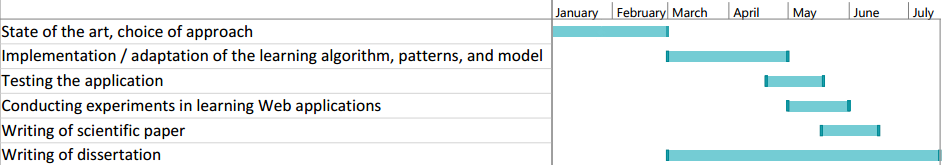
\includegraphics[width=\textwidth]{gantt_en}
  \end{center}
   \caption{Gantt chart representing the proposed work plan.}
  \label{fig:gantt}
\end{figure}

As of the moment of the writing of this article, the research on both the state of the art regarding reverse engineering approaches, learning algorithms and the familiarization process with the PARADIGM-RE tool will carry on being done until the ending of February. Following these steps, the effective work is then ready to be started, comprising a phase which should last until roughly the end of April. By then, the work developed thus far will undergo a learning phase (realization of experiences on learning GUIs, for the learning algorithm to draw conclusions on heuristics) and a testing and validation phase (of the newly developed patterns identified, the XMI model production and of the heuristics gotten via the learning algorithm, respectively) making adjustments as needed. This phase is expected to be concluded until the month of May at most. \\
This early deadline aims to make time to write a scientific paper, as well as to wrap up the dissertation document, which will be progressing in parallel with the previous phases. All the work here detailed is expected to be done by June of the current year.